\documentclass[a4paper]{article}

\documentclass[a4paper]{article}
\usepackage[utf8]{inputenc}
\usepackage[spanish, es-tabla, es-noshorthands]{babel}
\usepackage[table,xcdraw]{xcolor}
\usepackage[a4paper, footnotesep = 1cm, width=20cm, top=2.5cm, height=25cm, textwidth=18cm, textheight=25cm]{geometry}
%\geometry{showframe}

\usepackage{tikz}
\usepackage{amsmath}
\usepackage{amsfonts}
\usepackage{amssymb}
\usepackage{float}
\usepackage{graphicx}
\usepackage{caption}
\usepackage{subcaption}
\usepackage{multicol}
\usepackage{multirow}
\setlength{\doublerulesep}{\arrayrulewidth}
\usepackage{booktabs}

\usepackage{hyperref}
\hypersetup{
    colorlinks=true,
    linkcolor=blue,
    filecolor=magenta,      
    urlcolor=blue,
    citecolor=blue,    
}

\newcommand{\quotes}[1]{``#1''}
\usepackage{array}
\newcolumntype{C}[1]{>{\centering\let\newline\\\arraybackslash\hspace{0pt}}m{#1}}
\usepackage[american]{circuitikz}
\usetikzlibrary{calc}
\usepackage{fancyhdr}
\usepackage{units} 

\graphicspath{{../Ejercicio-1/}{../Ejercicio-2/}{../Ejercicio-3/}{../Ejercicio-4/}}

\pagestyle{fancy}
\fancyhf{}
\lhead{22.01 Teoría de Circuitos}
\rhead{Mechoulam, Lambertucci, Rodriguez Turco, Londero, Galdeman}
\rfoot{\centering \thepage}

\usepackage{float}
\usepackage{graphicx}

\begin{document}

\subsection{Diseño del circuito}

En el siguiente punto se propuso como objetivo realizar un sensor de temperatura, valiéndose del uso del transistor LM35. Este dispositivo se caracteriza por entregar a la salida una tensión proporcional a la temperatura dada la ecuación
\[
	V_{LM35} = 35 \frac{mV}{^{\circ}C} \ T
\]

De esta forma, se busca que el circuito diseñado posea una tensión de salida de $ 0 \ V $ A $ 35 ^{\circ}C $ y $ 5 \ V $ A $ 45 ^{\circ}C $. Es así que se busca que la tensión de salida sea regida por la ecuación

\begin{equation}
	V_{out} = 50V_{LM35} - 17.5 \ V =  1.75 \frac{V}{^{\circ}C} \ T - 17.5 \ V
	\label{equ:sistema}
\end{equation}

Para este, se seleccionaron dos amplificadores operacionales TL072 y un diodo zener \textbf{PONER NOMBRE DEL ZENER}.

Teniendo en cuenta lo ya mencionado, se decidió realizar un circuito con tres etapas que permita realizar lo deseado.
La primer etapa consiste en un amplificador operacional conectado como un inversor, cuya tensión de entrada es la de salida del transistor. De esta forma se logra que $V_1 = -5 V{LM35}$.

\begin{figure}[H]
	\centering
	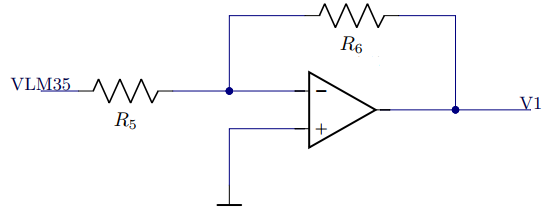
\includegraphics[width=0.8\textwidth]{Ejercicio6/Imagenes/CircuitoEtapa1-M1.png}
\caption{Primera etapa del circuito.}
	\label{fig:cir1-M1}
\end{figure}

En la segunda etapa se encuentra conformada nuevamente por un operacional, pero en este caso, conectado como un amplificador restador. Se alimenta dicho circuito con la tensión $V_1$, es decir, la salida de la primer etapa, al borne negativo del operacional, y con una tensión de $- 10 \ V$ al positivo.

\begin{figure}[H]
	\centering
	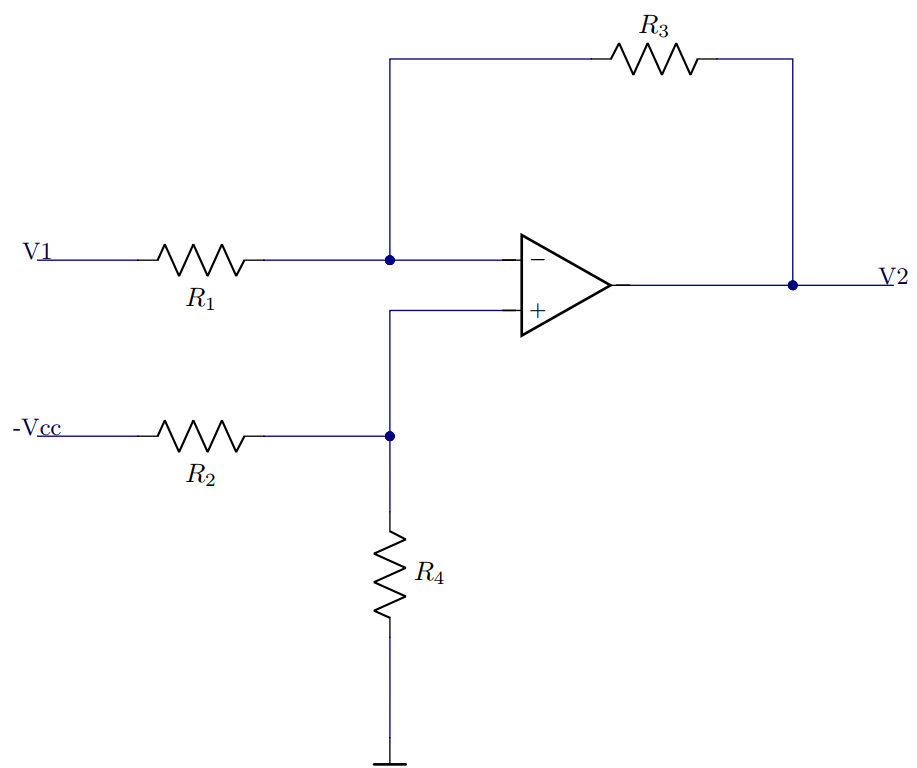
\includegraphics[width=0.8\textwidth]{Ejercicio6/Imagenes/CircuitoEtapa2-M1.png}
	\caption{Segunda etapa del circuito.}
	\label{fig:cir2-M1}
\end{figure}

Finalmente, la tercer etapa, consiste simplemente en una resistencia con un diodo zener en serie, cumpliendo la función de limitar la salida entre $-0,7 \ V$ y $5.6 \ V$, cumpliendo con las especificaciones deseadas de que la tensión de salida no sea menor a $-1 \ V$ ni mayor a $6 \ V$. La resistencia de protección colocada a la entrada de esta parte del circuito fue calculada ...

\begin{figure}[H]
	\centering
	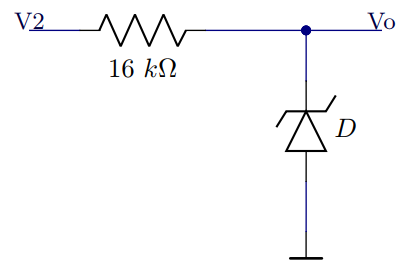
\includegraphics[width=0.6\textwidth]{Ejercicio6/Imagenes/CircuitoEtapa3-M1.png}
	\caption{Tercer etapa del circuito.}
	\label{fig:cir3}
\end{figure}

Es así como se observa al circuito final en la Figura (\ref{fig:cirfin-M1}).

\begin{figure}[H]
	\centering
	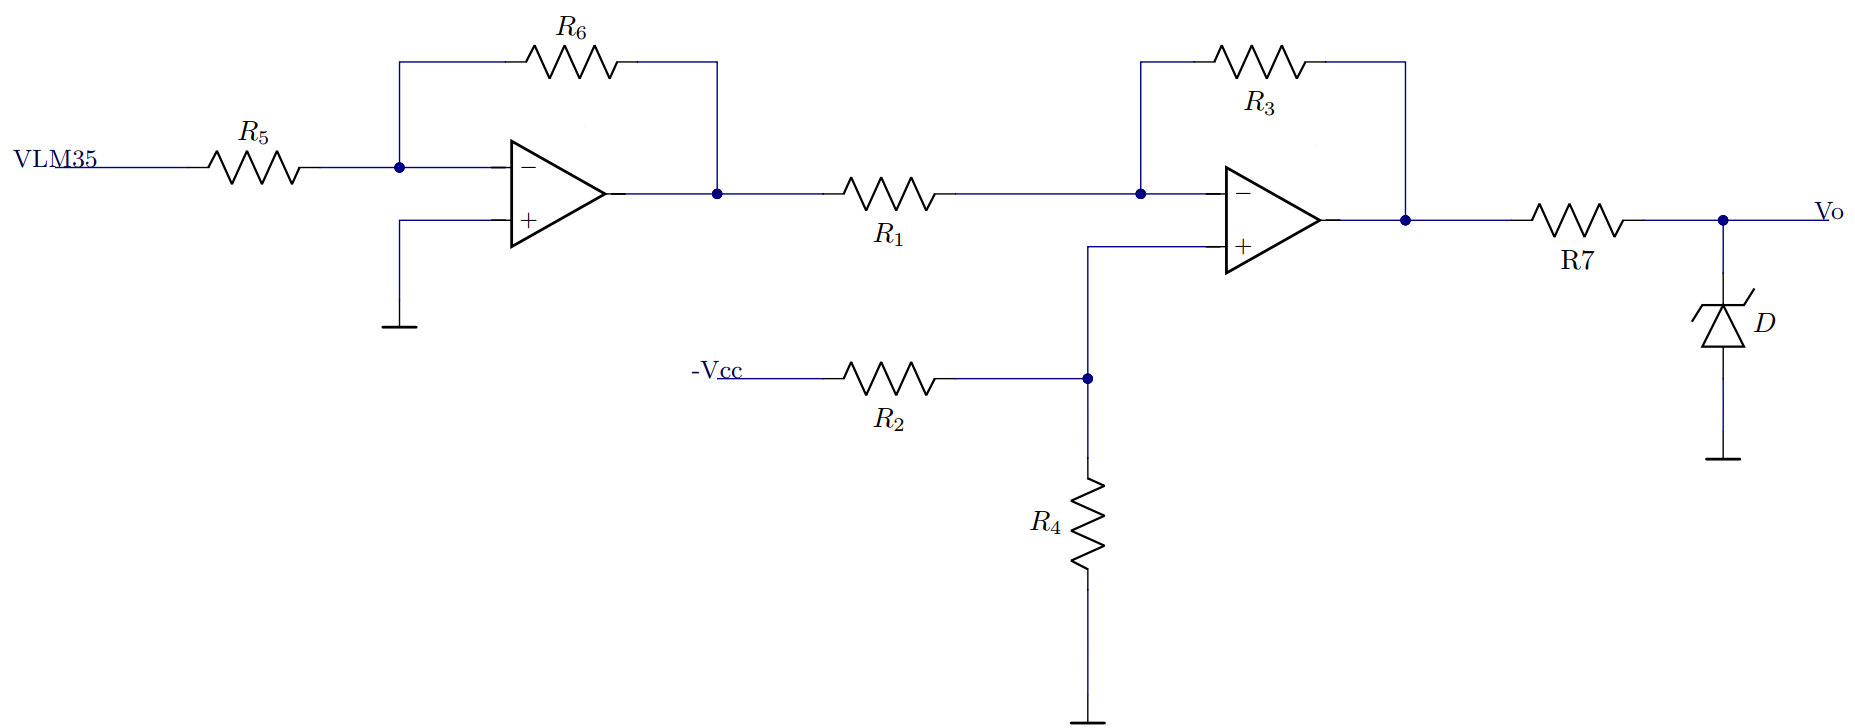
\includegraphics[width=0.9\textwidth]{Ejercicio6/Imagenes/CircuitoFinal-M1.png}
	\caption{Modelo final del circuito.}
	\label{fig:cirfin-M1}
\end{figure}

\subsection{Modo de uso}
%alimentacion, lectura, calibracion


\subsection{Detalles técnicos}
%Mediciones, corrientes/tensiones maximas, rango de temperatura, 

%El LM35 es un circuito integrado cuya tensi´on de salida var´ıa linealmente con la temperatura. Se desea que la
%se~nal pueda ser adquirida por un sistema con (por ejemplo, un conversor anal´ogico/digital) con tensi´on de entrada
%variable entre 0V y 5V .
%a. Dise~nar un circuito utilizando el LM35 que adapte la se~nal para que pueda ser adquirida con m´axima excursi´on
%para temperaturas que var´ıen entre 35◦C y 45◦C (35◦C ! 0V − 45◦C ! 5V ).
%b. Implementar el circuito en placa multiperforada o PCB.
%c. Dise~nar un m´etodo de calibraci´on del circuito para que se cumpla la especificaci´on.
%d. El circuito debe contar con una protecci´on de forma tal de que la tensi´on de salida no se encuentre por debajo
%de −1V ni por encima de 6V .
%e. Incluir en el informe un datasheet de la implementaci´on final, incluyendo toda la informaci´on relevante.


\end{document}